\documentclass[11pt]{article}
\usepackage[utf8]{inputenc}
\usepackage{algorithm}
\usepackage{graphicx}
\usepackage{mathtools}
\usepackage{amsmath}
\usepackage{amsfonts}
\usepackage{hyperref}
\usepackage{geometry}
\usepackage{multicol}
\usepackage{capt-of}
\usepackage{url}
\usepackage[italian]{babel}
\geometry{a4paper, top=2.5cm, bottom=2.5cm, left=3cm, right=3cm, bindingoffset=5mm}
\usepackage[suftesi]{frontespizio}

\title{Relazione di Laboratorio - Condensatore, Induttore, Cavo Coassiale ed Equazioni Differenziali}
\author{Nicolò Favagrossa C.M. 969124\\nicolo.favagrossa@studenti.unimi.it\\}
\date{Giugno 2022}
\begin{document}

\maketitle
\newpage
\tableofcontents
\newpage
\section{Introduzione}
Lo scopo di questa relazione è introdurre in modo riassuntivo ma completo le principali funzionalità e teoria che stanno dietro a due fondamentali componenti dell'elettronica: il condensatore e l'induttore. Attraverso un semplice circuito sarà possibile risolvere un'equazione differenziale non omogenea del primo ordine. Oltre a questo si procede con la descrizione e lo studio di un cavo coassiale di tipo BNC lungo $100\,m$. Il fenomeno principale dell'esperimento è la carica e la scarica del condensatore e dell'induttore che si può studiare visualizzando nell'oscilloscopio la differenza di potenziale in uscita dal circuito detto circuito R-C (nel caso del conduttore) e circuito R-L (nel caso dell'induttore). Gli obiettivi dell'esperienza svolta in laboratorio sono:
\begin{itemize}
    \item verificare sperimentalmente la scarica del condensatore e dell'induttore su una resistenza;
    \item studiare il comportamento del condensatore attraverso il derivatore attivo;
    \item studiare il condensatore come by-pass in frequenza;
    \item realizzare un circuito analogico che risolve una equazione differenziale non omogenea del primo ordine;
    \item studiare il cavo coassiale.
\end{itemize}
\section{Trattazione Teorica}
\subsection{Condensatore}
Il condensatore è formato da due superfici conduttrici, detti elettrodi, poste una davanti all'altra. I due elettrodi, quando si lavora con un condensatore, vengono chiamati armature. Le due armature sono separate da un isolante che può essere l'aria o da un altro dielettrico che caratterizza la capacità del condensatore. Si può scrivere la seguente equazione che indica l'esistenza di una proporzionalità diretta tra la carica presente sulle superfici e la differenza di potenziale tra le armature:
\begin{equation}
    Q=CV
    \label{qcv}
\end{equation}
Dove $Q$ è la carica, $C$ è la capacità del condensatore e $V$ e la differenza di potenziale. 

Successivamente se svolgo la derivata temporale nell'equazione (\ref{qcv}), si ottiene:
\begin{equation}
    \frac{d}{dt}Q=C\frac{d}{dt}V \quad \Longrightarrow \quad i(t)=C\frac{dV}{dt}
\end{equation}
e così si trova l'equazione del condensatore. Analizzando i risultati trovati, se in un circuito con un condensatore si applica un segnale costante nel tempo, le derivate si annullano portando a: $i(t)=0$. Questo risultato si traduce sperimentalmente con il fatto che i condensatori bloccano correnti e differenze di potenziali costanti nel tempo. Questo non accade con segnali variabili nel tempo, ad esempio con una forma sinusoidale. Per verificarlo si può risolvere un semplice circuito R-C composto solo da un condensatore e una resistenza.
\newpage
\subsection{Circuito C-R}
Dall'immagine sottostante si può visualizzare schematicamente il circuito (\ref{RC}) in cui si devono invertire la posizione del condensatore e della resistenza per ottenere il circuito C-R.
Sperimentalmente in un primo momento si può studiare il comportamento del circuito fornendo una differenza di potenziale costante nel tempo e successivamente utilizzare un generatore di funzione per generare una tensione variabile nel tempo. Partendo dall'equazione di Kirchhoff alla maglia:
\begin{equation}
   \begin{cases}
   V_{in}=V_C+V_R\\ V_R=Ri \\ \dfrac{dV_C}{dt}=\dfrac{i}{C}
   \end{cases}
\end{equation}
Sostituendo e risolvendo la prima equazione si ottiene:
\begin{equation}
    \frac{dV_{in}}{dt}=\frac{dV_C}{dt}+\frac{dV_R}{dt} \quad \Rightarrow \quad \frac{dV_{in}}{dt}=\frac{i}{C}+R\frac{di}{dt}
    \label{gg}
\end{equation}
Ottenendo un'equazione differenziale che lega la corrente e la differenza di potenziale varabile nel tempo (altrimenti tutte le derivate si annullerebbero).

Ipotizzando che sia la $V_{in}$ che la corrente $i$ abbia una forma sinusoidale:
\begin{equation}
    V_{in}=V\sin(\omega t) \qquad \qquad i=I\sin(\omega t + \phi)
\end{equation}
Sostituendo la $V_{in}$ e la $i$ all'interno dell'equazione (\ref{gg}) si ottiene:
\begin{equation}
    V\omega\cos(\omega t)=\frac{I}{C}\sin(\omega t + \phi)+RI\omega\cos(\omega t+\phi)
    \label{q}
\end{equation}
E derivandola rispetto al tempo:
\begin{equation}
    -V\omega^2\sin(\omega t)=\frac{I}{C}\omega\cos(\omega t +\phi)-RI\omega^2\sin(\omega t+\phi)
    \label{t}
\end{equation}
Sommando le due equazioni (\ref{q}) + (\ref{t}) e dopo vari passaggi si arriva alla soluzione:
\begin{equation}
    I=\frac{\omega C}{\sqrt{1+R^2C^2\omega^2}}V
    \label{I}
\end{equation}
Di conseguenza l'ipotesi fatta in precedenza per la corrente è confermata da questo risultato. Inoltre, l'ultima equazione ottenuta ci fornisce informazioni anche sull'ampiezza dell'onda sinusoidale di corrente di maglia del circuito C-R. Come si può notare dall'equazione (\ref{I}), l'ampiezza della corrente di maglia dipende dall'ampiezza della $V_{in}$ e dalla frequenza angolare che sto fornendo alla sinusoide di ingresso. Infatti se idealmente si fa tendere $\omega$ ad infinito ($\omega \to \infty$) l'equazione (\ref{I}) tende a diventare la legge di Ohm e cioè: $I=V/R$. Da questo risultato si può concludere che ad alte frequenze il condensatore si comporta come un corto circuito, mentre a basse frequenze il condensatore si comporta come un circuito aperto. Per alte frequenze si intende: $\omega >> 1/RC$, infatti $RC$ ha le dimensioni di un tempo.

Imponendo $t=0$ nell'equazione (\ref{t}) si ottiene la fase $\phi$:
\begin{equation}
    \phi=\arctan\left(\frac{1}{\omega RC}\right)
    \label{p}
\end{equation}
Infine, utilizzando la legge di Ohm si può calcolare la tensione di uscita del circuito R-C:
\begin{equation}
    V_R(t)=Ri(t)=RI\sin(\omega t+\phi)
\end{equation}
dove $I$ e $\phi$ sono ricavabili dalle relazioni: (\ref{I}) e (\ref{p}). 

Utilizzando ciò che si è appena appreso riguardo il condensatore si può studiare il fenomeno di carica e scarica del condensatore nel circuito R-C. Risolvendo le equazioni esposte in precedenza si ottiene che la scarica del condensatore ha un andamento di tipo esponenziale decrescente:
\begin{equation}
    V_{out}(t)=Ve^{-\frac{t}{RC}}
\end{equation}

\subsection{Derivatore attivo}
Il circuito rappresentato schematicamente nell'immagine (\ref{der}) permette di misurare la corrente che fluisce sui fili delle armature del condensatore. Infatti è sufficiente misurare la sua differenza di potenziale utilizzando l'oscilloscopio. Risolvendo le equazioni:
\begin{equation}
   \begin{cases}
   i_r=i_c\\ V_{out}=-V_{R} \\ V_{R}=i_RR \\ V_C=V_{in}
   \end{cases}
\end{equation}
si ottiene:
\begin{equation}
    V_{out}(t)=-Ri_C(t)=-RC\frac{dV_C}{dt}=-RC\frac{dV_{in}}{dt}
    \label{corr}
\end{equation}
Ipotizzando di inserire nel circuito una differenza di potenziale variabile nle tempo, ad esempio con una forma sinusoidale $V_{in}=V\sin(\omega t)$ utilizzando l'equazione (\ref{corr}) si ricava l'equazione della differenza di potenziale che in laboratorio misuro con l'oscilloscopio:
\begin{equation}
    V_{out}(t)=-RCV2\pi f\cos(2\pi f t)
    \label{cp}
\end{equation}
Da cui ricavo la corrente del condensatore dividendo la tensione $V_{out}(t)$ per $R$ e cambiando di segno:
\begin{equation}
    i_C(t)=\frac{V_R}{R}=\frac{-V_{out}}{R}=CV2\pi f \cos(2\pi f t)
\end{equation}
Da cui si nota la proporzionalità diretta tra la corrente (analogamente anche per la differenza di potenziale) e la frequenza della sinusoide che si inietta dentro il circuito.

\begin{figure}[htp!]
  \centering
  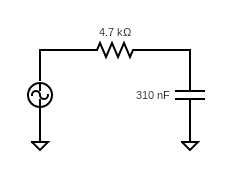
\includegraphics[scale=0.6]{RC.png} \quad 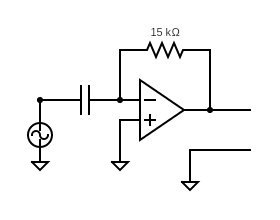
\includegraphics[scale=0.6]{derivatore.png}
  \caption{Nello schema a sinistra è rappresentato il circuito R-C. Il generatore fornisce una differenza di potenziale in funzione del tempo: un'onda quadra. Nello schema a destra, invece, è rappresentato il circuito usato per studiare le caratteristiche del condensatore al variare della frequenza della $V_{in}$. Il generatore fornisce una differenza di potenziale in funzione del tempo: un'onda sinusoidale.}
  \label{RC}
  \label{der}
\end{figure}
\newpage
\subsection{Induttore}
Un induttore è un componente elettronico costituito da $N$ spire avvolte di materiale conduttivo ricoperto da una sottile pellicola isolante. Prendendo in considerazione una singola spira ($N=1$) ed utilizzando la legge di Biot e Savart si può calcolare il campo magnetico e il suo flusso, infatti al centro della spira si ottiene:
\begin{equation}\begin{split}
|\Vec{B}|=\frac{\mu}{2R}i\\
\Phi_B=L_1i
\end{split}\end{equation}
Dove $\mu$ rappresenta la permeabilità magnetica del materiale con cui è composto il nucleo. Da come si può notare dalla formula del flusso esiste una proporzionalità diretta tra il flusso del campo magnetico $\Phi_B$ e la corrente $i$ regolata dall'induttanza $L$. Applicando la legge di Faraday-Lenz si ottiene la forza elettromotrice e quindi una differenza di potenziale tra il punto di ingresso e di uscita della singola spira:
\begin{equation}
    f.e.m.=-\frac{\partial\Phi_B}{\partial t}=-L_1\frac{\partial i}{\partial t}
\end{equation}
Considerando ora un induttore con $N$ spire il flusso del campo magnetico totale diventa:
\begin{equation}
    \Phi_B=\mu\frac{N^2}{l}Si=L_Ni
\end{equation}
Dove $l$ è la lunghezza del solenoide ed $S$ l'area della singola spira. Con il flusso, come si è appena visto nel caso di una singola spira si può ricavare la $f.e.m.$ e l'induttanza:
\begin{equation}
   \begin{cases}
   f.e.m.=-L_N\dfrac{\partial i}{\partial t}\\ L_N=\dfrac{\mu N^2 S}{l}
   \end{cases}
   \label{L}
\end{equation}
Trovando l'equazione dell'induttore. Risulta importante notare che il segno della legge di Faraday-Lenz dipende dalla convezione usata. In elettronica l'equazione della $f.e.m.$ che è composta dall'induttanza e dalla derivata parziale della corrente rispetto al tempo è con il segno più. 
\subsection{Circuito L-R}
Attraverso il circuito L-R, mostrato schematicamente nell'immagine (\ref{LR}), si può sperimentare e verificare cosa succede se applico una differenza di potenziale agli estremi di un induttore. Dalla teoria è noto il fatto che c'è un periodo transitorio in cui la differenza di potenziale in entrata è "contrastata" dalla presenza della $f.e.m.$. Infatti dalla legge di Faraday-Lanz la corrente generata dall'induttore si oppone alla causa. Di conseguenza si studia la carica e la scarica dell'induttore. Per quanto riguarda il fenomeno di scarica, dall'equazione di Kirchhoff alla maglia si ottengono le seguenti relazioni:
\begin{equation}
   \begin{cases}
   V_{out}(t)=Ri(t)\\ V_{out}(t)=-V_L(t) \\ V_L(t)=L\dfrac{di}{dt}
   \end{cases}
\end{equation}
Facendo vari passaggi algebrici si ottiene un'equazione differenziale:
\begin{equation}
    \frac{di}{dt}=-\frac{R}{L}i(t)
\end{equation}
Di cui una soluzione è:
\begin{equation}
    i(t)=ke^\frac{-t}{L/R}
\end{equation}
Dove $k$ (imponendo le condizioni iniziali $i(0)=V/R$) è $k=V/R$. Si sta studiando quindi un decadimento di tipo esponenziale che decade con un tempo dettato dalla relazione $L/R$.

Infine essendo che $V_{out}(t)=Ri(t)$ ottengo:
\begin{equation}
    V_{out}(t)=Ve^\frac{-t}{L/R}
    \label{Ind}
\end{equation}
\begin{figure}[htp!]
\centering
  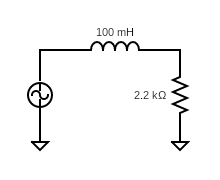
\includegraphics[scale=0.7]{LR.png}
  \caption{In questo schema è rappresentato il circuito L-R. Il generatore fornisce una differenza di potenziale in funzione del tempo: un'onda quadra.}
  \label{LR}
  \end{figure}
\subsection{Circuito per la risoluzione delle equazioni differenziali non omogenee di primo ordine}
Attraverso i concetti appena introdotti è possibile costruire un circuito che permette di risolvere un'equazione differenziale del primo ordine. La branca dell'elettronica che si occupa di risolvere problemi di questo tipo è detta analogica. Come si può osservare dallo schema del circuito (\ref{difffere}), è sostanzialmente un circuito R-C collegato ad un buffer a guadagno unitario tramite un amplificatore operazionale. Il buffer serve ad evitare di perturbare la misura dell'uscita e quindi ridurre al minimo gli effetti di carico. Ipotizzando che $V=V_{in}\sin(\omega_0t)$ e passando alle equazioni:
\begin{equation}
   \begin{cases}
   V=V_R+V_C\\ i=C\dfrac{dV_C}{dt} \\ V_R=iR=RC\dfrac{dV_C}{dt} \\ V_{out}=V_C
   \end{cases}
   \label{s}
\end{equation}
Ottendendo:
\begin{equation}
    V_{in}=RC\dfrac{dV_{out}}{dt}+V_{out}
\end{equation}
In questa maniera ho un'equazione differenziale del primo ordine non omogenea la cui soluzione ha i seguenti parametri:
\begin{equation}\begin{split}
V_{out}=\frac{V_{in}}{\sqrt{1+(\omega_0 RC)^2}}\\
\phi=\tan^{-1}(\omega_0 RC)
\label{Solut}
\end{split}\end{equation}
\begin{figure}[htp!]
\centering
  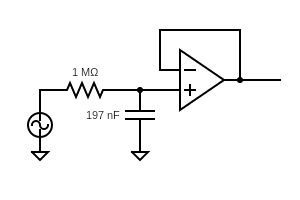
\includegraphics[scale=0.7]{diffe.png}
  \caption{In questo schema è rappresentato il circuito usato per risolvere l'equazione differenzale non omogenea di primo ordine. Il generatore produce una differenza di potenziale variabile nel tempo (ad esempio a forma sinusoidale) mentre l'uscita è la soluzione dell'equazione.}
  \label{difffere}
  \end{figure}
\subsection{Cavo Coassiale}
Il cavo coassiale è un sistema fisico utilizzato per trasmettere segnali elettrici di vario tipo. Come primo esempio, il cavo coassiale viene ampiamente utilizzato per trasmettere il segnale delle antenne televisive fino ai nostri televisori. Per studiare le caratteristiche fisiche del cavo coassiale è necessario schematizzarlo, in prima approssimazione, come una catena infinita di celle elementari con una componente induttiva e una componente capacitiva (L-C) di lunghezza infinitesima. Utilizzando $C$ come capacità per unità di lunghezza $[F/m]$ e $L$ l'induttanza per unità di lunghezza $[H/m]$ possiamo applicare le equazioni dell'induttore e del condensatore. Per quanto riguarda l'equazione dell'induttore:
\begin{equation}
    dV=Ldx\frac{\partial }{\partial t}(i+di)\approx Ldx\frac{\partial i}{\partial t} \quad \Rightarrow \quad \frac{\partial V}{\partial x}=L\frac{\partial i}{\partial t} \quad \Rightarrow \quad \frac{1}{L}\frac{\partial^2V}{\partial x^2}=\frac{\partial ^2i}{\partial t\partial x}
    \label{V}
\end{equation}
Applicando ora l'equazione del condensatore
\begin{equation}
    di=Cdx\frac{\partial V}{\partial t} \quad \Rightarrow \quad \frac{\partial i}{\partial x}=C\frac{\partial V}{\partial t}\quad \Rightarrow \quad \frac{\partial^2i}{\partial x\partial t}=C\frac{\partial^2V}{\partial t^2}
    \label{i}
\end{equation}
Eguagliando le due relazioni si ottiene l'equazione di d'Alembert:
\begin{equation}
    \frac{\partial^2V}{\partial x^2}=LC\frac{\partial^2V}{\partial t^2}
\end{equation}
L'equazione di d'Alambert descrive il comportamente di propagazione delle onde. Di conseguenza il sistema fisico in esame che si ha all'interno del cavo coassiale è un'onda di tensione (ma si potrebbe anche esprimere la stessa equazione per la corrente) che si propaga con una velocità:
\begin{equation}
    v=\frac{1}{\sqrt{LC}}=\frac{c}{\sqrt{\varepsilon_r}}
    \label{v}
\end{equation}
Il fatto che una superficie equipotenziale abbia un tempo $t$ che dipende dalla velocità di propagazione in cui non è equipotenziale in tutta la superficie è necessario dalla relativià. Infatti se una superficie infinitamente estesa messa a contatto con una carica $Q$ raggiungesse istantaneamente l'equipotenzialità significherebbe che l'informazione (in questo caso di carica) si è propagata più velocemente della luce. 

Un altro risultato molto importante di queste due equazioni si ricava facendo il rapporto tra l'equazione (\ref{V}) e l'equazione (\ref{i}) ottendendo:
\begin{equation}
    \frac{dV}{di}=\sqrt{\frac{L}{C}}
    \label{imp}
\end{equation}
Che ha le dimensioni di una resistenza. Questa quantità è chiamata impedenza caratteristica del cavo. 
\section{Procedure e Dati Sperimentali}
\subsection{Scarica del condensatore}
L'obiettivo principale delle esperienze in laboratorio è quella di verificare la compatibilità tra lo studio teorico e le misure sperimentali. Ci proponiamo quindi di osservare sperimentalmente attraverso l'oscilloscopio la scarica esponenziale del condensatore con il circuito rappresentato schematicamente nell'immagine (\ref{RC}). E' necessario:
\begin{multicols}{2}
\begin{itemize}
    \item Condensatore da $310\,nF$;
    \item resistenza da $4.7\,k\Omega$;
    \item oscilloscopio;
    \item generatore $33220A$.
\end{itemize}
\end{multicols}
Dopo aver costruito il circuito, attraverso il generatore di funzione bisogna fornire un'onda quadra $V_{PP}$ di $0.5\,V$ con frequenza $50\,Hz$. Successivamente aggiustando il range dell'oscilloscopio si riesce a visualizzare in maniera completa il caratteristico andamento esponenziale della scarica del consensatore. Successivamente grazie al software OSC è stato possibile campionare l'andamento su excel ottenendo il seguente grafico (\ref{Scex}).





\begin{figure}[htp!]
\centering
  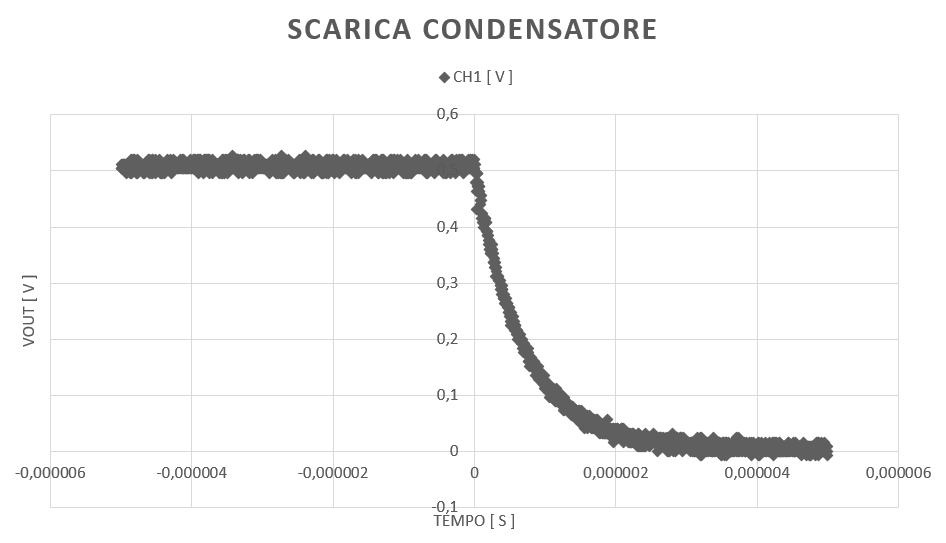
\includegraphics[scale=0.4]{ScaricaEx.png}
  \caption{In questo grafico si può visualizzare il caratteristico andamento esponenziale della scarica del condensatore campionato in laboratorio.}
  \label{Scex}
  \end{figure}
\begin{table}[ht]
    \centering
    \begin{tabular}{|c|c|c|}
    \hline
     $C\,[nF]$ & $R\,[k\Omega]$ & $1/(RC)\,[s^{-1}]$ \\
    \hline
    $310\pm62$ & $4.7\pm0.3$ & $684.53\pm144.09$ \\
    \hline
    \end{tabular}
    \caption{In questa tabella sono riportati i valori della resistenza $R$, del condensatore $C$ ed infine la costante di decadimento $1/(RC)$. $R$ è fornita con una tolleranza del $5\%$ mentre $C$ del $20\%$. Mentre l'errore associato alla costante di decadimento è stata ricavata tramite propagazione degli errori.}
    \label{datConde}
\end{table}
\newpage
Svolgendo il fit dei dati attraverso MATLAB ho ottenuto i seguenti risultati: (\ref{FitC}).
\begin{figure}[htp!]
\centering
  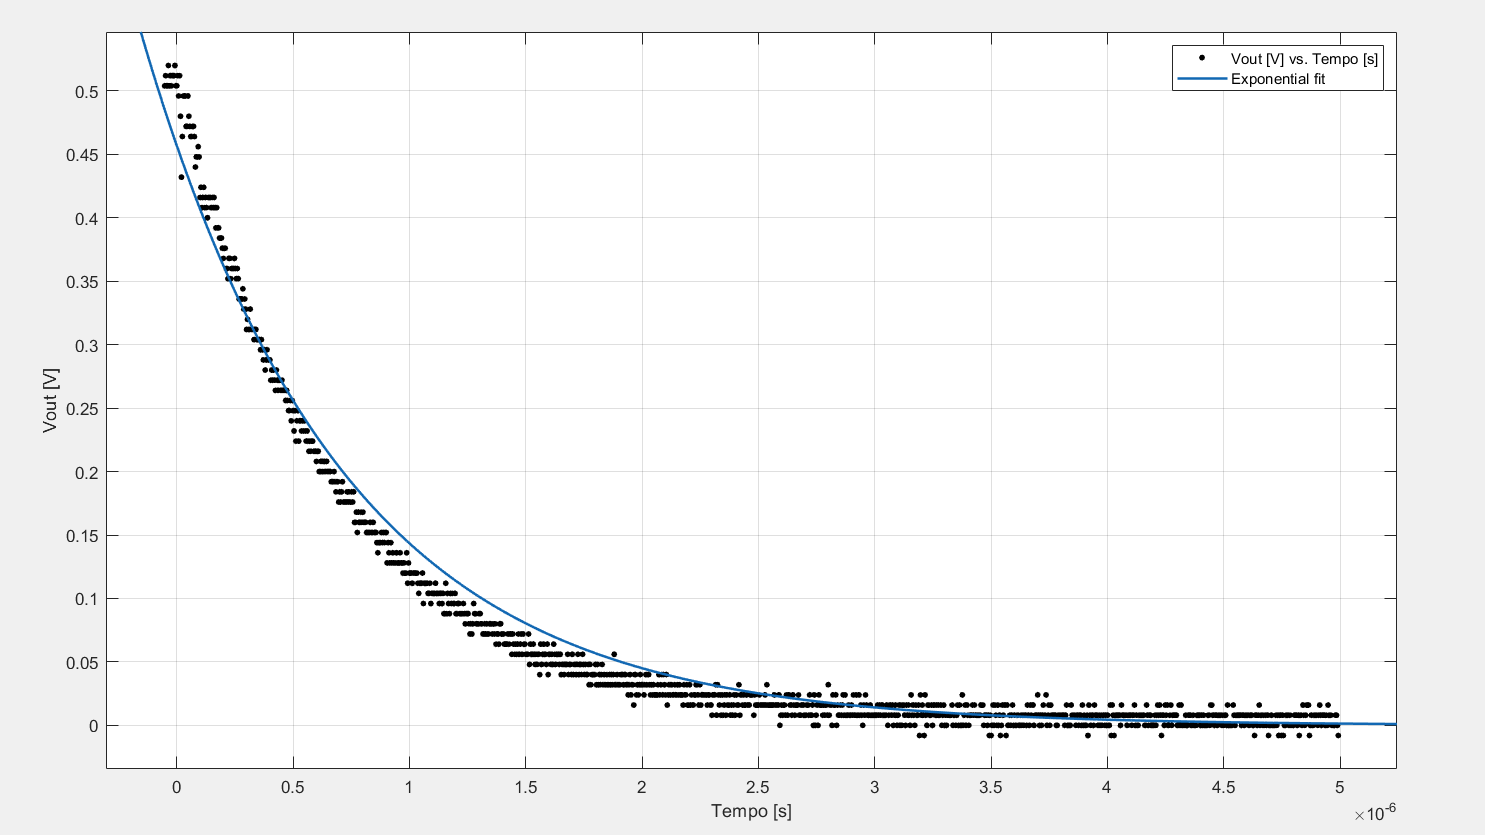
\includegraphics[scale=0.2]{fitcond.png}
  \caption{In questo grafico si può visualizzare l'andamento dei dati sperimentali che rappresentano la scarica del condensatore e la linea di tendenza che rappresenta l'andamento esponenziale.}
  \label{FitC}
  \end{figure}
Questo grafico rappresenta un andamento esponenziale del tipo :$f(t)=a\,exp(bt)$. I dati che si ottengono attraverso il fit sono:
\begin{equation}
   \begin{cases}
   a=0.4569\\ b=-1.159\times10^{6}
   \end{cases}
\end{equation}
Confrontando $1/RC$ e il coefficiente libero $b$ si nota in maniera qualitativa un'enorme discrepanza tra le due grandezze. Un motivo plausibile potrebbe essere causato da un'errata impostazione del generatore o dell'oscilloscopio. 

Per studiare invece quantitativamente la compatibilità della distribuzione dei dati sperimentali con l'andamento esponenziale, MATLAB calcola in maniera automatica il coefficiente R-squared.
\begin{equation}
    R-squared =0.9842
\end{equation}
Che indica una perfetta relazione fra il fenomeno analizzato e l'andamento atteso dalla teoria.

\subsection{Studio del Condensatore}
In questa sezione si andrà ad esporre lo studio e la misura della corrente che fluisce in un condensatore quando su di esso viene impostata una differenza di potenziale variante. Successivamente si verifica che il condensatore blocca la corrente continua, mentre "lascia passare" come corrente di spostamente la corrente alternata ad alta frequenza. Di seguito un elenco di tutto l'occorrente:
\begin{multicols}{2}
\begin{itemize}
    \item Due condensatori da $470\, pF$ e $1\,uF$;
    \item resistenza da $15\,k\Omega$;
    \item amplificatore operazionale;
    \item due alimentatori da $\pm12\,V$ presente sull'IDL-800;
    \item generatore $33220A$;
    \item oscilloscopio.
\end{itemize}
\end{multicols}
Dopo aver costruito il circuito presente in figura (\ref{der}), si imposta il generatore di funzioni per produrre un'onda sinusoidale con un'ampiezza picco-picco da $500\,mV$. Successivamente è necessario studiare e misurare l'ampiezza di uscita dal circuito al variare della frequenza della sinusoide tra $1\,kHz$ e $200\,Hz$. Attraverso le equazioni presentate nella trattazione teorica si può verificare che la dipendenza tra la differenza di potenziale (o la corrente con un fattore moltiplicativo) ha una dipendenza lineare con la frequenza della sinusoide di ingresso.
Ora, inserendo i dati misurati in laboratorio in un grafico in cui è rappresentato il guadagno in funzione della frequenza e usando la scala logaritmica nelle ascisse e nelle ordinate si ottiene il seguente risultato atteso e predetto dalla teoria (\ref{frecc}).
\begin{figure}[htp!]
\centering
  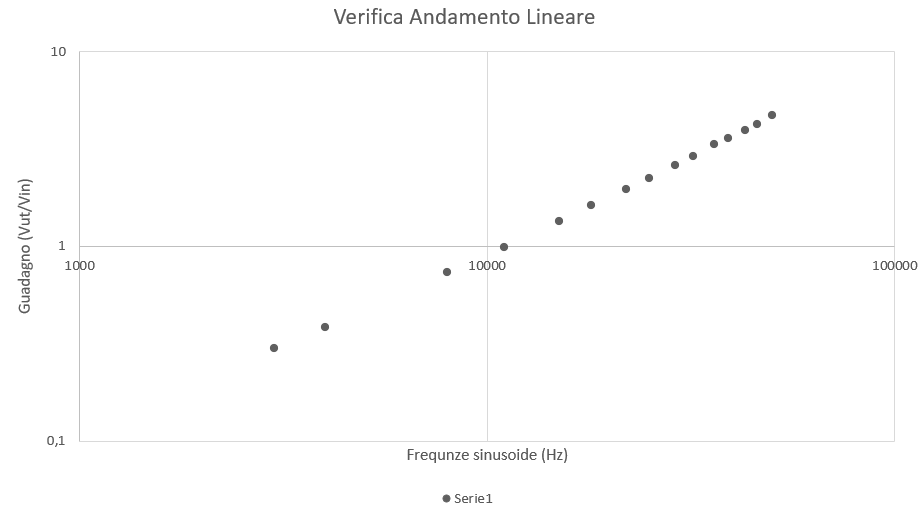
\includegraphics[scale=0.4]{frequenzcond.png}
  \caption{In questo grafico è rappresentato il guadagno in funzione della frequenza in scala logaritmica. L'andamento è qualitativamente lineare come previsto dalla teoria.}
  \label{frecc}
  \end{figure}
Il fenomeno che descrive il grafico rappresenta il fatto che l'ampiezza della sinusoide di uscita tende a crescere al crescere della frequenza. Attraverso l'equazione (\ref{cp}) si può calcolare la $V_{out}$ attesa e confrontarla con quella misurata in laboratorio. Di seguito riporto la tabella con i valori della frequenza, del guadagno, di $V_{teo}$ e di $V_{spe}$ avendo come costante $V_{in}=0.5\,V$.
\begin{table}[ht]
    \centering
    \begin{tabular}{|c|c|c|c|}
    \hline
     $f\,[Hz]$ & $V_{out}/V_{in}$ & $V_{spe}\,[V]$ & $V_{teo}\,[V]$\\
    \hline
    $3000$ & $0.15$ & $0.075$ & $0.066$ \\
    $4000$ & $0.19$ & $0.096$ & $0.087$ \\
    $8000$ & $0.37$ & $0.184$ & $0.174$ \\
    $11000$ & $0.5$ & $0.248$ & $0.241$ \\
    $15000$ & $0.67$ & $0.334$ & $0.328$ \\
    $18000$ & $0.81$ & $0.404$ & $0.393$ \\
    $22000$ & $0.99$ & $0.492$ & $0.481$ \\
    $25000$ & $1.12$ & $0.56$ & $0.546$ \\
    $29000$ & $1.3$ & $0.65$ & $0.634$ \\
    $32000$ & $1.44$ & $0.72$ & $0.7$ \\
    $36000$ & $1.66$ & $0.83$ & $0.787$ \\
    $39000$ & $1.8$ & $0.9$ & $0.852$ \\
    $43000$ & $1.96$ & $0.98$ & $0.94$ \\
    $46000$ & $2.12$ & $1.06$ & $1.01$ \\
    $50000$ & $2.34$ & $1.17$ & $1.09$ \\
    \hline
    \end{tabular}
    \caption{In questa tabella è possibile visualizzare in maniera immediata il confronto tra i dati sperimentali e i valori teorici. Inoltre, è analogo lo studio della corrente in quanto varia solo di un fattore moltiplicativo costante.}
    \label{prev}
\end{table}

Successivamente bisogna costruire il circuito rappresentato schematicamente nell'immagine (\ref{RC}) invertendo la posizione delle due componenti elettroniche formando così il circuito C-R. Per prima cosa bisogna verificare che iniettando una differenza di potenziale costante, l'uscita, misurabile dall'oscilloscopio sia nulla. Dopodichè, si imposta dal generatore di funzione un'onda sinusoidale e si campiona l'uscita del circuito al variare della frequenza dell'onda di ingresso. Di seguito, è presente il grafico del guadagno in funzione della frequenza della sinusoide di ingresso:
%Più tabella (FREQUENZA; GUADAGNO; VOUT)
\begin{figure}[htp!]
\centering
  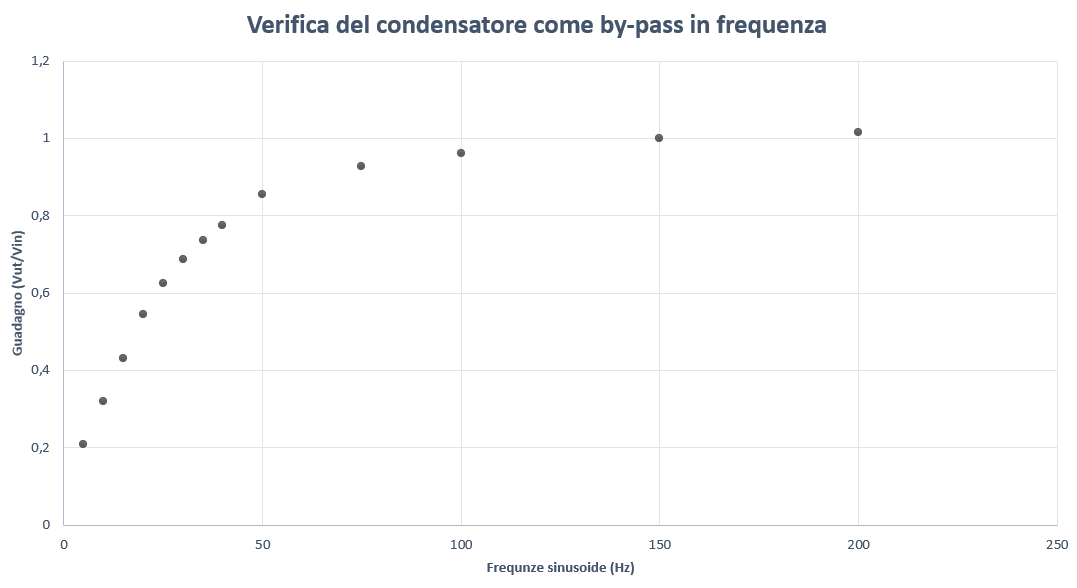
\includegraphics[scale=0.4]{bypass.png}
  \caption{In questo grafico è rappresentato il guadagno in funzione della frequenza. Come è previsto dalla teoria a frequenze in un intorno di $5\,Hz$ il condensatore si comporta come un circuito aperto. Mentre a frequenze intorno a $200\, Hz$ si comporta come un cortocircuito.}
  \label{byp}
  \end{figure}
\subsection{Risoluzione dell'equazione differenziale del primo ordine}
Dopo aver studiato il circuito rappresentato schematicamente nell'immagine (\ref{difffere}) è possibile risolvere un'equazione differenziale non omogenea del primo ordine. Per farlo è necessario:
\begin{multicols}{2}
\begin{itemize}
    \item Resistenza da  $1\,M\Omega$;
    \item condensatore da $197\,nF$;
    \item oscilloscopio;
    \item generatore $33220A$;
    \item amplificatore operazionale;
    \item due alimentatori da $\pm12\,V$ presente sull'IDL-800.
\end{itemize}
\end{multicols}
Il primo passo è assemblare il circuito in modo corretto e collegare il generatore di funzioni come ingresso e l'oscilloscopio come uscita del circuito. Successivamente ho imposto una differenza di potenziale variabile nel tempo con una forma sinusoidale con $V_{PP}=5\,V$ e una frequenza di $5\,Hz$. Usando uno sdoppiatore a forma di "T" ho sdoppiato il segnale di uscita del generatore in modo tale da visualizzare nell'oscilloscopio i due canali: nel canale 1 è possibile visualizzare la $V_{in}$ mentre nel secondo canale è possibile visualizzare la $V_{out}$. Riporto di seguito il grafico campionato in laboratorio (\ref{difi}).
\begin{figure}[htp!]
\centering
  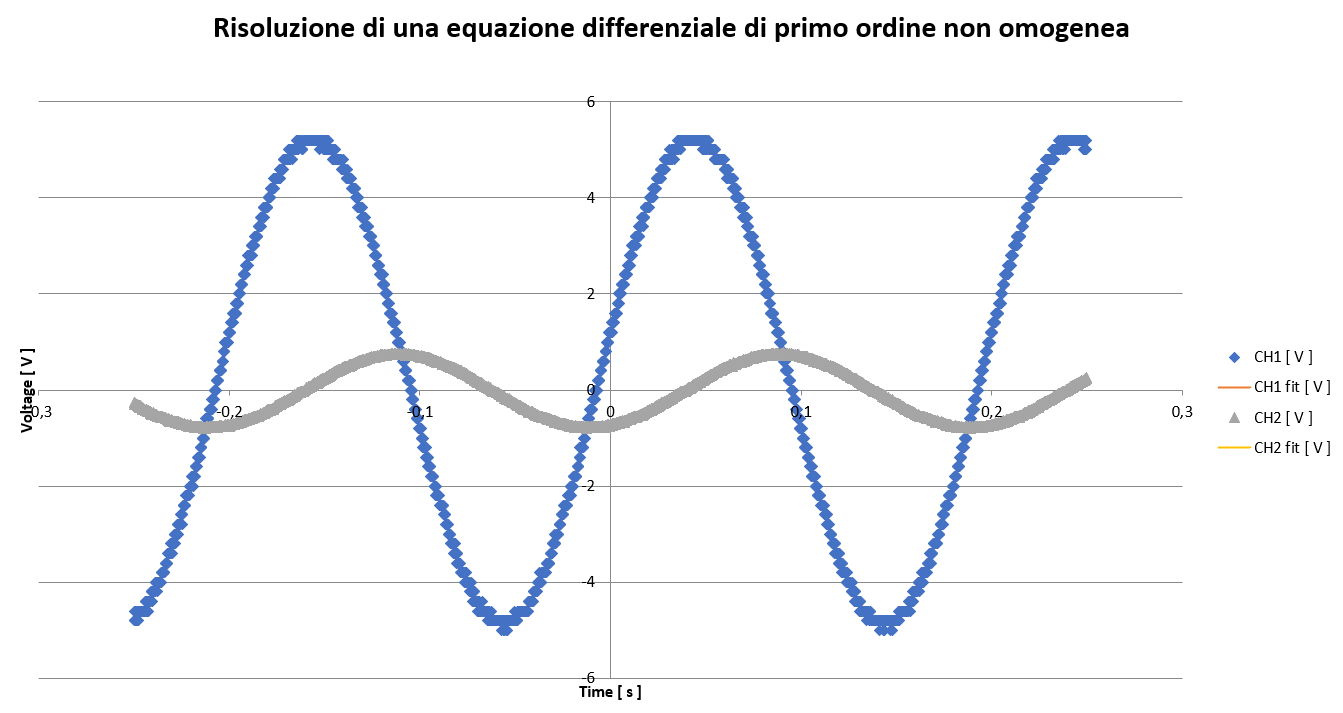
\includegraphics[scale=0.35]{dffer.png}
  \caption{In questo grafico si può visualizzare in modo chiaro il campionamento dei due canali dell'oscilloscopio. Il canale 1 rappresenta l'onda sinusoidale di ingresso, il canale 2 rappresenta l'onda sinusoidale di uscita del circuito che secondo la teoria dovrebbe essere la soluzione dell'equazione differenziale non omogenea del primo ordine presentata nella sezione di trattazione teorica.}
  \label{difi}
  \end{figure}
  
  
  Di seguito riporto una tabella che contiene i valori misurati e i valori teorici calcolati attraverso le relazioni (\ref{Solut}):
\begin{table}[ht]
    \centering
    \begin{tabular}{|c|c|c|c|}
    \hline
     $V_{spe}\,[V]$ & $V_{teo}\,[V]$ & $\phi_{spe}$ & $\phi_{teo}$\\
    \hline
    $0.880$ & $0.798$ & $1.583$ & $1.411$ \\
    \hline
    \end{tabular}
    \caption{In questa tabella è possibile visualizzare le misure sperimentali e i dati teorici per quanto riguarda l'ampiezza e la fase della sinusoide di uscita}
    \label{datdiff}
\end{table}

Per descrivere in maniera quantitativa la bontà dei risultati ottenuti sarebbe stato indicativo riuscire a campionare più punti e quindi essere in grado di misurare più differenze di tempo e di conseguenza più fasi. In questa maniera si sarebbe potuto svolgere un test di compatibilità tra i valori sperimentali e i valori teorici attraverso il test t di student. Ora l'unico modo è quello di calcolare semplicemente la discrepanza delle misure dai valori teorici senza fare supposizioni concrete ma solo qualitative sulla riuscita dell'esperimento.
\begin{equation}\begin{split}
D_V=|V_{teo}-V_{spe}|=0.082\\
D_\phi=|\phi_{teo}-\phi_{spe}|=0.172
\end{split}\end{equation}
\subsection{Scarica dell'Induttore}
In questa sezione si presentano i dati ottenuti in laboratorio studiando la scarica dell'induttore (fenomeno descritto nella sezione di trattazione teorica). Come strumentazione si è utilizzato:
\begin{multicols}{2}
\begin{itemize}
    \item Un induttore da $10\, mH$;
    \item una resistenza da $2.2 \,k\Omega$;
    \item generatore $33220A$;
    \item oscilloscopio.
\end{itemize}
\end{multicols}
Per riuscire a campionare in modo completo l'uscita del circuito si è collegato l'oscilloscopio al computer presente in laboratorio, che grazie ad un software scritto in Phyton riesce a campionare ogni punto presente a schermo dello strumento elettronico. Dopo aver montato il circuito presente schematicamente nell'immagine (\ref{LR}) e svolti tutti i collegamenti si imposta il generatore per produrre un'onda quadra con un'altezza di: $V_{PP}=0.5\,V$ e con una frequenza pari a: $f=50\,Hz$. Il risultato dell'esperienza è raffigurato nel grafico (\ref{dx}) in cui si può visualizzare l'andamento esponenziale della scarica dell'induttore. 

\begin{figure}[htp!]
\centering
  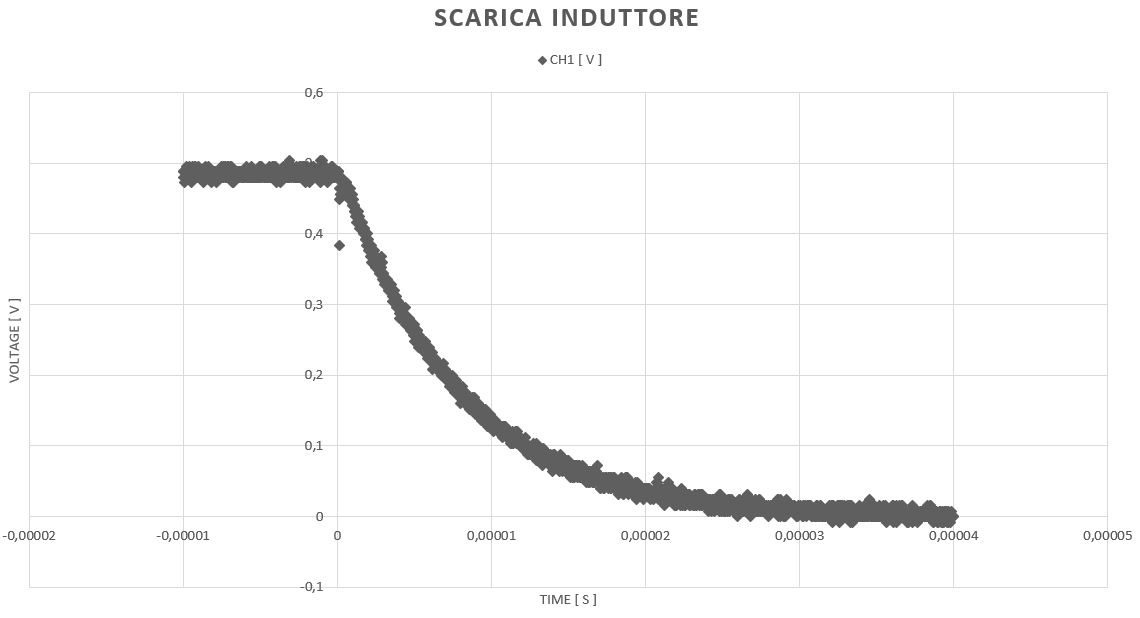
\includegraphics[scale=0.28]{patma.png}
  \caption{In questo grafico si può visualizzare il caratteristico andamento esponenziale della scarica del'induttore campionato in laboratorio.}
  \label{dx}
  \end{figure}



L'andamento esponenziale è descritto dall'equazione (\ref{Ind}).
\begin{table}[ht]
    \centering
    \begin{tabular}{|c|c|c|}
    \hline
     $L\,[H]$ & $R\,[\Omega]$ & $1/(L/R)\,[s^{-1}]$ \\
    \hline
    $0.010\pm0.002$ & $(2.20\pm0.11)\times10^3$ & $(2.2\pm 0.5)\times10^{5}$ \\
    \hline
    \end{tabular}
    \caption{In questa tabella sono riportati i valori della resistenza $R$, dell'induttore $L$ ed infine la costante di decadimento $1/(L/R)$ con relative incertezze. L'incertezza relativa alla resistenza e all'induttore è rispettivamente del $5\%$ e del $10\%$. L'incertezza relativa alla costante di decadimento è stata ricavata tramite propagazione degli errori. }
    \label{datInd}
\end{table}
Utilizzando il software MATLAB si può eseguire un fit e valutare quantitativamente la compatibilità dei dati ottenuti. Di seguito allego l'immagine del fit con i relativi risultati:
\begin{figure}[htp!]
\centering
  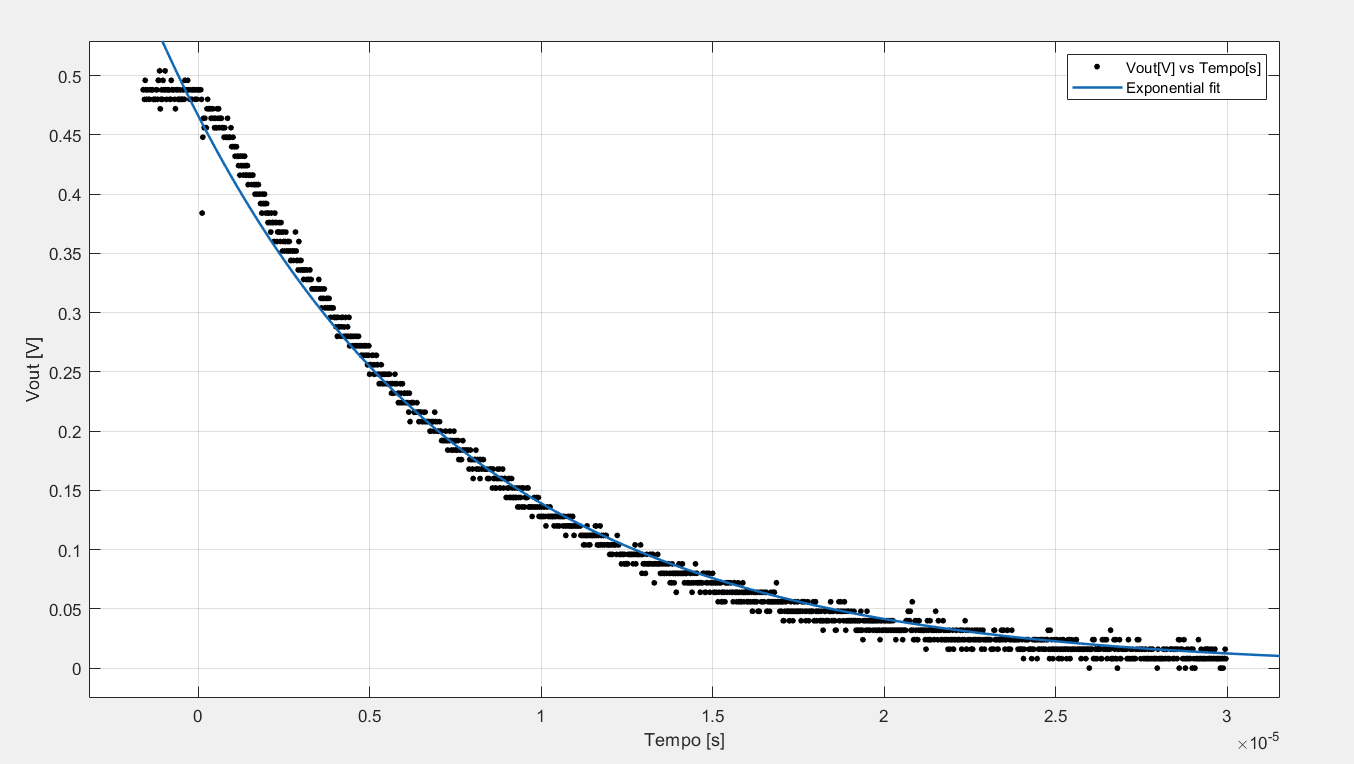
\includegraphics[scale=0.2]{indutscar.png}
  \caption{In questo grafico si può visualizzare l'andamento dei dati sperimentali che rappresentano la scarica dell'induttore e la linea di tendenza che rappresenta l'andamento esponenziale.}
  \label{FitI}
  \end{figure}
  
  
  Questo grafico rappresenta un andamento esponenziale del tipo :$f(t)=a\,exp(bt)$. I dati che si ottengono attraverso il fit sono:
\begin{equation}
   \begin{cases}
   a=0.4665\\ b=-1.21\times10^{5}
   \end{cases}
\end{equation}
Per studiare invece quantitativamente la compatibilità della distribuzione dei dati sperimentali con l'andamento esponenziale, si calcola il coefficiente di determinazione:
\begin{equation}
    R-squared =0.991
\end{equation}
Che indica una perfetta relazione fra il fenomeno analizzato e l'andamento atteso dalla teoria.
\subsection{Cavo coassiale: propagazione e misura di parametri fisici}
Di seguito un elenco degli strumenti utilizzati durante questa esperienza:
\begin{multicols}{2}
\begin{itemize}
    \item Cavo coassiale BNC da $50\,\Omega$ di impedenza lungo $100\,m$;
    \item oscilloscopio;
    \item generatore $33220A$;
    \item resistenza da $50\,\Omega$.
\end{itemize}
\end{multicols}
Come primo esperimento si propone di misurare la velocità di propagazione del segnale elettrico all'interno del cavo BNC. Per fare ciò si propone di terminare il cavo con una resistenza da $50\,\Omega$ tra il centrale del cavo e il suo schermo ad una estremità del cavo stesso. Successivamente bisogna iniettare un segnale ad onda quadra con il generatore di funzione sull'altra estremità. Grazie ad uno sdoppiatore è stato possibile collegare direttamente due canali all'oscilloscopio e cioè la funzione iniettata all'inizio del cavo e la funzione di arrivo dopo che il segnale ha attraversato l'intero filo. In questo modo è stato possibile misurare la differenza tra un picco di una onda quadra e l'altro per ricavare il tempo di propagazione del segnale stesso. Di seguito è presente il campionamento dei due canali dell'oscilloscopio (\ref{cav}). 
\begin{figure}[htp!]
\centering
  
\includegraphics[scale=0.4]{dsa.png}
  \caption{In questo grafico si può visualizzare l'onda quadra iniettata all'ingresso del cavo coassiale (canale 2) e l'uscita (canale 1)}
  \label{cav}
  \end{figure}
  


Le misure effettuate sono quindi:
\begin{table}[ht]
    \centering
    \begin{tabular}{|c|c|c|}
    \hline
     $\Delta t\,[ns]$ & $L\,[m]$ & $v_p\,[ms^{-1}]$ \\
    \hline
    $508$ & $100$ & $1.97\times10^{8}$ \\
    \hline
    \end{tabular}
    \caption{In questa tabella sono presenti i valori misurati in laboratorio e la velocità di propagazione del segnale elttrico calcolata tramite la lunghezza del cavo e il tempo di sfasamento tra l'onda quadra iniettata e l'onda quadra nel capo opposto del cavo.}
    \label{datCav}
\end{table}


Il segnale si dovrebbe propagare ad una velocità di circa $v_{teo}\approx\frac{2}{3}c$. Quindi imponendolo come dato teorico si ottiene una larga compatibilità con il dato sperimentale. %mancano errori e compatibilità
Successivamente, per come è costituito il cavo BNC, è possibile misurare la capacità per unità di lunghezza attraverso le due equazioni (\ref{v}) e (\ref{imp}):
\begin{equation}
    C=\frac{1}{v_pZ}=102\,\frac{pF}{m}
\end{equation}
Dove $Z$ è l'impedenza caratteristica del cavo coassiale. Infine è possibile anche ricavare la costante dielettrica relativa $\varepsilon_r$ della guaina isolante interna al cavo attraverso l'equazione (\ref{v}) ottenendo:
\begin{equation}
    \varepsilon_r=\frac{c^2}{v_p^2}=2.32\,\frac{C^2}{Nm^2}
\end{equation}

Dal grafico è anche possibile visualizzare il corretto comportamento dell'onda in quanto la presenza della resistenza da $50\,\Omega$ dovrebbe eliminare gran parte dell'eco che si verificherebbe se non ci fosse una terminazione in arrivo.

Nel secondo esperimento si propone di studiare il comportamento del segnale all'interno del cavo nel caso di circuito aperto. Per effetto eco, nel caso di cirucito aperto in arrivo, si verifica un'interferenza costruttiva tra onda avanzante e onda retrocedente come si può visualizzare nel grafico (\ref{cav1}):
\begin{figure}[htp!]
\centering
  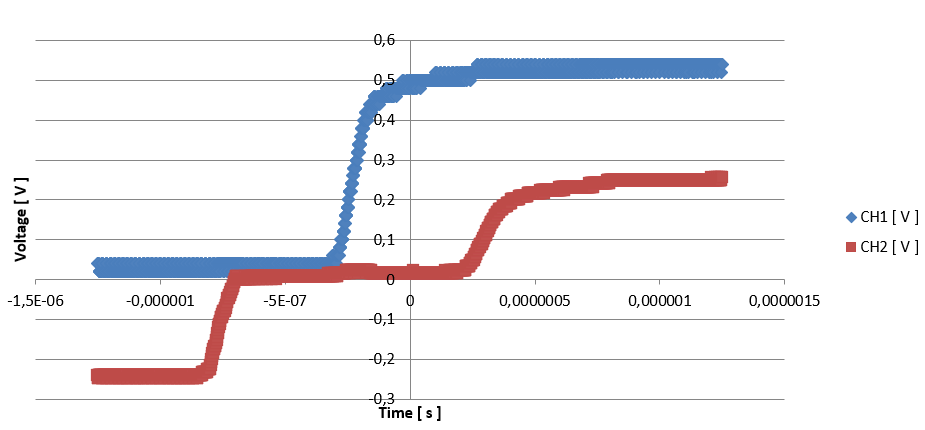
\includegraphics[scale=0.4]{sdf.png}
  \caption{In questo grafico si può visualizzare l'onda quadra iniettata all'ingresso del cavo coassiale (canale 2) e l'uscita (canale 1).}
  \label{cav1}
  \end{figure}
Dal grafico è possibile visualizzare in modo chiaro il doppio picco del canale 2 in quanto per effetto eco si ha un fenomeno di interferenza costruttiva che raddoppia l'ampiezza dell'onda.
\section{Conclusione}
Ricapitolando, l'obiettivo dell'esperienza è presentare in modo completo la teoria e il funzionamento di due fondamentali componenti elettronici: il condensatore e l'induttore. Il primo set di esperimenti vede come protagonista il condensatore. Dopo aver introdotto tutte le formule utilizzate per prevedere il comportamento dei vari circuiti si è studiato il fenomeno di scarica del condensatore. Il circuito utilizzato è visualizzabile nell'immagine (\ref{RC}) mentre i risultati sperimentali campionati in laboratorio sono stati studiati e interpretati a partire dal grafico (\ref{Scex}). Utilizzando MATLAB è stato possibile effettuare un fit esponenziale per verificare la compatibilità della distribuzione misurata con l'andamento previsto dalla teoria. Successivamente utilizzando il circuito detto derivatore attivo (\ref{der}) si è semplicemente verificato che il guadagno del circuito fosse direttamente proporzionale alla frequenza imposta dal generatore di funzione (\ref{frecc}). Ritornando al circuito C-R si è studiato il comportamento del condensatore quando viene fornita una differenza di potenziale variabile nel tempo a diverse frequenze. L'andamento ottenuto coincide con le ipotesi teoriche svolte: il condensatore si comporta come un circuito aperto a basse frequenze mentre come un corto circuito ad alte frequenze (\ref{byp}).

Risolvendo l'equazione alla maglia del circuito (\ref{difffere}) si ottiene un'equazione differenziale la cui soluzione può essere ottenuta campionando l'uscita attraverso un'oscilloscopio visualizzabile nel grafico (\ref{difi}). I risultati sono stati studiati solo in maniera qualitativa perchè non disponevo di abbastanze misure per effettuare un test di compatibilità ragionevole.

Si è poi passato a studiare l'induttore. Analogamente allo studio del condensatore si è studiato il fenomeno di scarica dell'induttore campionando le misure in laboratorio ed ottenendo il grafico (\ref{dx}). In maniera equivalente al processo di analisi dati della scarica del condensatore si è svolto un fit dei dati attraverso MATLAB (\ref{FitI}).

Come ultimo sistema fisico si è studiato il cavo coassiale di tipo BNC. Quest'ultimo è composto, in prima approssimazione, da celle capacitive e induttive. Il primo esperimento consiste nel studiare il comportamento del cavo in caso di terminazione con una resistenza da $50\Omega$ che impedisce il formarsi di effetti eco non desiderati (\ref{cav}). Successivamente si è misurato l'intervallo di tempo che separa il primo e il secondo canale e successivamente la velocità di propagazione del segnale $V_p=1.97\times10^8\,ms^{-1}$. Attraverso varie relazioni è stato possibile calcolare anche la capacità parassita del cavo e la costate dielettrica relativa: $C=102\,pFm^{-1}$ e $\varepsilon_r=2.32\,C^2N^{-1}m^{-2}$. Infine si è studiato il comportamento del segnale in caso il cavo coassiale abbia come terminazione il circuito aperto (\ref{cav1}).
\end{document}


